\documentclass[12pt]{scrreprt}
\usepackage{graphicx} % Required for inserting images
\usepackage[top=2.5cm, bottom=2.5cm, left = 2cm, right = 2cm]{geometry}
\geometry{a4paper}
\usepackage[utf8]{inputenc}
\usepackage{amsmath,amssymb}
\usepackage[pdftex,bookmarks,colorlinks,breaklinks]{hyperref}
\hypersetup{linkcolor=blue,citecolor=red,filecolor=black,urlcolor=black}
%\setlength{\headheight}{12pt}
\usepackage{times,subcaption,pdfpages}
\usepackage{listings}
\usepackage{float}
\linespread{1}
%\setlength{\parskip}{0.5em}
\usepackage{booktabs}
\usepackage[style=nature,backend=biber]{biblatex}
\usepackage{sectsty}
\chapterfont{\centering}
\sectionfont{\centering}

\begin{document}


\begin{titlepage}
   \begin{center}
       \large
       \vspace*{1cm}

       \textbf{ME5627 Measurements in Thermofluids }

       \vspace{0.5cm}
       
       \textbf{Laboratory Record}
       
       \vspace{6cm}

       \textbf{Submitted By\\~\\}
       {Rakesh S S 132414011 \\Vimal S V 132404001}


       \vspace{4cm}
     
       {
\includegraphics[width=4.5cm]{logos/iitpkd_fulllogo_color.pdf} \\}
       
       \vspace{2cm}   
       
       Department Mechanical Engineering\\
       Indian Institute of Technology Palakkad

       %\today           
   \end{center}
\end{titlepage}
\newpage

\chapter*{\normalsize EXPERIMENT 1}
\setcounter{chapter}{1}
\section*{\normalsize PART A: FAMILIARISATION WITH PC SCOPE AND BREAD BOARD THROUGH
RC CIRCUIT}
\textbf{Aim} – To gain familiarity with Bread Board, oscilloscope and oscilloscope data logger through RC circuit\\
\\
\textbf{Apparatus} – Bread board, wires, Oscilloscope, Resistor, capacitor\\
\\
\textbf{Details of Bread Board:}

\begin{figure}[H]
    \centering
    \begin{subfigure}[b]{0.6\textwidth}
        \centering
        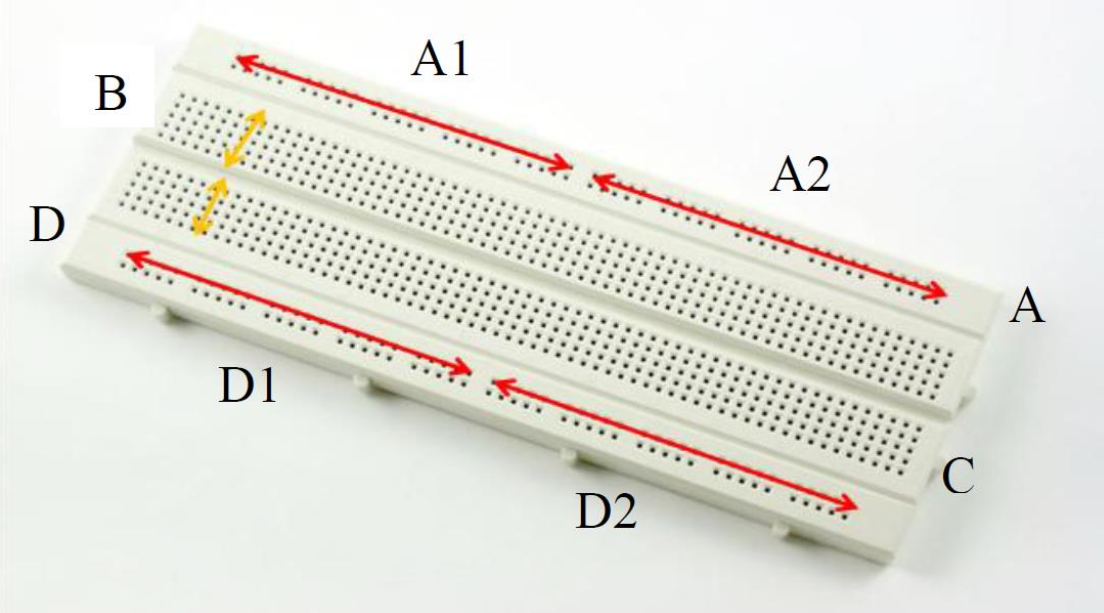
\includegraphics[width=\linewidth]{logos/Breadboard.png}
        \caption{Schematic of the Bread Board}
        \label{fig:Breadboard}
    \end{subfigure}
    \\
    \begin{subfigure}[b]{0.45\textwidth}
        \centering
        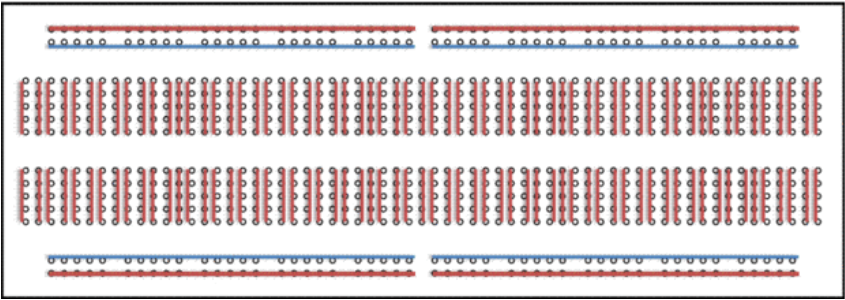
\includegraphics[width=\textwidth]{logos/Breadboard_connections.png}
        \caption{Equipotential lines}
        \label{fig:Breadboard_connections}
    \end{subfigure}
    \caption{Breadboard familiarisation}
    \label{fig:Breadboard familiarisation}
\end{figure}

\begin{itemize}
\item Hold the breadboard such that the horizontal side is longer than the vertical side.
\item There are four independent portions (A, B, C and D) created by three notches as in Fig.~\ref{fig:Breadboard}. Here, independence means portions A, B, C and D are not connected with each other
\end{itemize}

\textbf{\textit{Portion A and D}}
\begin{itemize}
\item Each portion of A and D is further subdivided into two regions as A1 and A2 shown in Fig.~\ref{fig:Breadboard familiarisation}.
\item Each horizontal line (shown through arrows in the Fig.~\ref{fig:Breadboard}) of A1, A2, D1 and D2 represent a single potential. Usually, as a general practice, these points are considered as ground for a given built circuit.
\end{itemize}

\textbf{\textit{Portion B and C}}
\begin{itemize}
\item In portion B and C, each vertical line (shown through arrows in Fig.~\ref{fig:Breadboard}) of B and C represents a single potential.
\item The above explanation can be better understood through Fig.~\ref{fig:Breadboard_connections} showing same potential lines.
\end{itemize}

\textbf{\textit{Details of oscilloscope probe}}\\

Fig.~\ref{fig:Oscilloscope_probe} shows a typical oscilloscope probe.

\begin{itemize}
\item The Oscilloscope probe is a passive connector which is used to connect oscilloscope to the electrical circuit. It consists of three parts Retractable hook tip (or crocodile clip), a Crocodile clip and BNC connector.
\item BNC connector: It is used to connect oscilloscope to the probe.
\item Retractable Hook tip: It is used to connect the node of the electrical circuit to the oscilloscope where there is a need to measure the signal.
\item Crocodile clip: It is connected to the ground of the electrical circuit in the bread board.
\item Make sure the RED slider on the probe should be on the X1 position only. X1 means amplification is unity.
\end{itemize}


\begin{figure}[H]
	\centering
	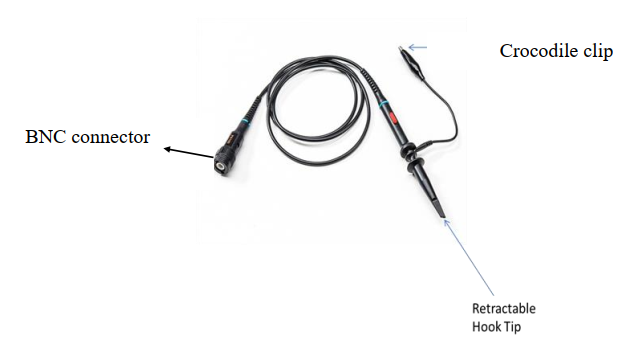
\includegraphics[width=0.8\linewidth]{logos/Oscilloscope_probe.png}
	\caption{PC scope probe}
	\label{fig:Oscilloscope_probe}
\end{figure}


Fig.~\ref{} shows a four channel Oscilloscope with digital data storage system. There are four
channels which displays the input/output signal. Input and output probes may be connected to any of these
four channels to visualize and analyze the waveforms of the signal. There are scaling, vertical and
horizontal controls to adjust the waveform in order to have better visualization. Peak to peak voltage and
time scale can be conveniently read from the monitor using the adjustment knob after pressing the cursor
button.

In order to obtain a desired input signal (sinusoidal, square, ramp, pulse or any arbitrary
waveform) a function generator can be used (Fig.~\ref{}). The desired amplitude and frequency of the
waveform can be obtained using the side controls near the monitor. The output probes may be connected
to any of the two channels. One of the crocodile clip of the output probe needs to be grounded and the
other end can be given as input signal to generate the signal in the circuit. Also, in order to check whether
the function generator is working, the probe may be connected to the Oscilloscope.

\textbf{Calculation of Resistance:}
\begin{itemize}
\item Turn the resistor so that the gold or silver stripe is at the right end of the resistor.
\item Look at the color of the first two stripes on the left end. These correspond to the first two digits
of the resistor value. Use the table given below to determine the first two digits.
\item Look at the third stripe from the left. This corresponds to a multiplication value. Find the value
using the table below.
\item Multiply the two digit number from step two by the number obtained from step three. This is the
value of the resistor in ohms. The fourth stripe indicates the accuracy of the resistor.
\end{itemize}

\textbf{Sample:}


You are given a resistor whose stripes are colored from left to right as brown, black, orange, gold. Find
the resistance value.
\begin{itemize}
\item The gold stripe is on the right so go to Step Two.
\item The first stripe is brown which has a value of 1. The second stripe is black which has a value of 0.
Therefore the first two digits of the resistance value are 10.
\item The third stripe is orange which means x 1,000.
\item The value of the resistance is found as 10 x 1000 = 10,000 ohms i.e., 10~k$\Omega$ 
\item The gold stripe means the actual value of the resistor may vary by $5\%$ meaning the actual value
will be somewhere between 9,500 ohms and 10,500 ohms. (Since $5\%$ of 10,000 = 0.05 x 10,000 = 500)
\end{itemize}

Calculation of Capacitance:
Sample Calculation:
\begin{itemize}
\item Step 1: In the Fig.~\ref{}, the first two digits from the left indicates the first two digits of the
capacitor value. Here, in this case the first two digits are 1 and 0. Therefore, the first two digits of
the capacitor value is 10.
\item Step 2: The third digit is 4 which means that four zeroes would be followed by 1 (10,000 pF).
\item The value of the capacitor is found out to be the product of the number obtained in step 1 and step
2. That is, 10 $\times$ 10000 = 10,0000 pF i.e 0.1 $\mu$F.
\end{itemize}
\chapter*{Experiment 2}
\end{document}